% !TEX encoding = UTF-8 Unicode
\documentclass[
10pt,
aspectratio=169,
]{beamer}
\setbeamercovered{transparent=10}
\usetheme[
  showheader,
%  red,
%  purple,
%  gray,
%  graytitle,
  colorblocks,
%  noframetitlerule,
]{Verona}

\usepackage[T1]{fontenc}
\usepackage[utf8]{inputenc}
\usepackage{lipsum}
\definecolor{col}{RGB}{0,68,158}
%%%%%%%%%%%%%%%%%%%%%%%%%%%%%%%
% Mac上使用如下命令声明隶书字体,windows也有相关方式,大家可自行修改
\providecommand{\lishu}{\CJKfamily{zhli}}
%%%%%%%%%%%%%%%%%%%%%%%%%%%%%%%
\usepackage{tikz}
\usetikzlibrary{fadings}
%
%\setbeamertemplate{sections/subsections in toc}[ball]
\usepackage{xeCJK}
\usepackage{listings}
\usepackage{caption}
\usepackage{subcaption}
\usefonttheme{professionalfonts}
\def\mathfamilydefault{\rmdefault}
\usepackage{amsmath}
\usepackage{multirow}
\usepackage{booktabs}
\usepackage{bm}
\usepackage{mathtools}
\usepackage{algorithm}
\usepackage{algpseudocode}
\setbeamertemplate{section in toc}{\hspace*{1em}\inserttocsectionnumber.~\inserttocsection\par}
\setbeamertemplate{subsection in toc}{\hspace*{2em}\inserttocsectionnumber.\inserttocsubsectionnumber.~\inserttocsubsection\par}
\setbeamerfont{subsection in toc}{size=\small}
%\AtBeginSection[]{%
%	\begin{frame}%
%		\frametitle{Outline}%
%		\textbf{\tableofcontents[currentsection]} %
%	\end{frame}%
%}

\AtBeginSubsection[]{%
	\begin{frame}%
		\frametitle{Table Of Contents}%
		\textbf{\tableofcontents[currentsection, currentsubsection]} %
	\end{frame}%
}

\title{Detection of transient signals in time series: application to gravitational wave data}
\subtitle{Introduzione alla Teoria Bayesiana della Probabilità}
\author[G.C.]{Giulio Cordova}
\mail{g.cordova@studenti.unipi.it}
\institute[Università di Pisa]{Dipartimento di Fisica E. Fermi\\
Università di Pisa}
\date{\today}
\titlegraphic[width=3cm]{cherubino_pant541}{}
%\definecolor{Veronagrayblue} {RGB}{0,91,129}
\newcommand\boldblue[1]{\textcolor{Veronagrayblue}{\textbf{#1}}}




%%%%%%%%%%%%%%%%%%%%%%%%%%%%%%%%
% ----------- 标题页 ------------
%%%%%%%%%%%%%%%%%%%%%%%%%%%%%%%%



\begin{document}

\maketitle


%%%%%%%%%%%%%%%%%%%%%%%%%%%%%%%%
% ----------- Temp ------------
%%%%%%%%%%%%%%%%%%%%%%%%%%%%%%%%

% \begin{exampleblock}{title}
% 		xxx
% 	\end{exampleblock}

% \begin{columns}[onlytextwidth]
% 		\begin{column}{.5\textwidth}
% 		\end{column}
% \end{columns}

% \begin{figure}
% 		\centering
% 		\includegraphics[width=0.8\linewidth]{fig/intro_private.png}
% 		\caption{Privacy security policy}
% \end{figure}

% \begin{equation*}
% 		w=\sum _{j=1}^{M}\frac{\left | \mathcal{D}_j \right | w_j^e}{\sum _{j=1}^{M}\left | \mathcal{D}_j \right |}
% \end{equation*}

%%%%%%%%%%%%%%%%%%%%%%%%%%%%%%%%
% ----------- FRAME ------------
%%%%%%%%%%%%%%%%%%%%%%%%%%%%%%%%


\section*{Overview}
\begin{frame}{Overview}
\boldblue{Aim:} detecting a gravitational wave signal in the noisy data stream of an interferometric detector
    \begin{figure}
        \centering
        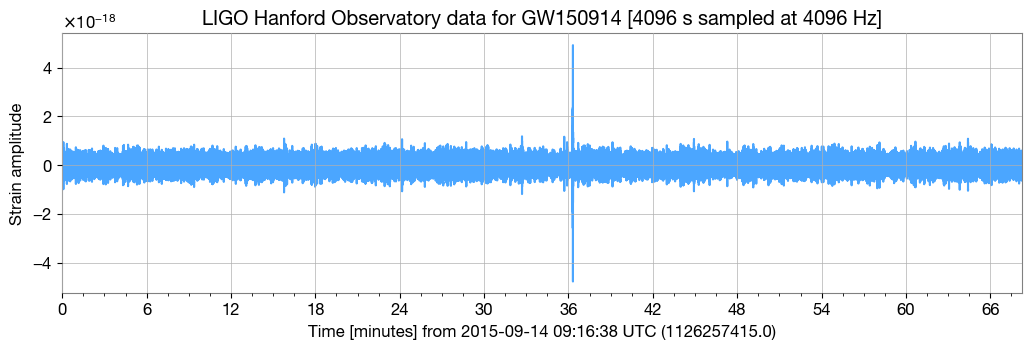
\includegraphics[width=\linewidth]{h1_strain_data.png}
       % \caption{H1 strain}
        %\label{fig:GW}
    \end{figure}
\end{frame}
\begin{frame}%
		\frametitle{Table Of Contents}%
		\textbf{\tableofcontents} %
	\end{frame}%
\section{Noise Modeling}
\subsection{Stochastic Processes}
\begin{frame}[c]{Discrete time stochastic process}
	
\begin{block}{Discrete time stochastic process}
	A discrete time stochastic process is a (possible infinite but still countable) sequence of random variables. Defining as $\nu(t)$ a random variable at time t, and as s the outcome of the
experiment, then 
\[\nu(t) = \phi(t,s) \quad \bigl( t \in \mathbb{Z}^+\bigr)\]
\end{block}
 \begin{columns}
           \column{0.33\linewidth}
             \begin{itemize}
 \item for time $t=\bar{t}$  fixed, $\phi$ is a random variable
 \vfill
 \item for $s = \bar{s}$ fixed, $\phi$ is a sequence of real numbers (realization of the stochastic process)
\end{itemize}
        \hfill
          \column{0.7\linewidth}
             \centering
             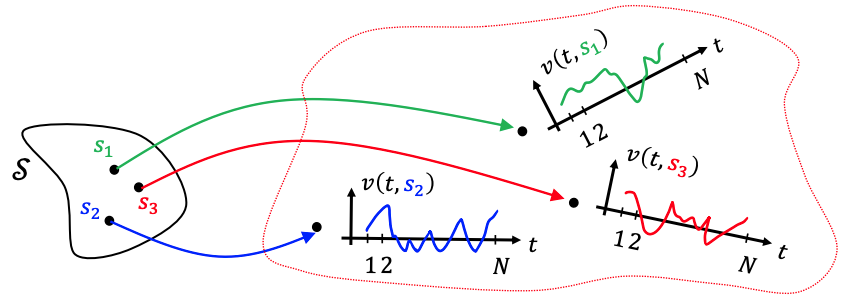
\includegraphics[height=0.4\textheight]{stoc_process.png}
         \end{columns} 
\end{frame}

\begin{frame}{Mean, autocovariance, ACF}

\begin{block}{Mean or expected value}
The mean is a function that represents the expected value of the random variable $\phi(t,s)$ at time $t$
	\[m(t) = \mathbb{E}_s[\phi(t,s)]  \] %= \frac{1}{n} \sum_{i=1}^{n} x_i(t)
\end{block}

\begin{block}{Autocovariance}
Let $\mu(t_i)$ be the expected value of $\phi(t_i,s)$ at time $t_i$, then the autocovariance matrix is defined as
	\[C(t_i,t_j) = \mathbb{E}_s[(\phi(t_i,s) - \mu(t_i))(\phi(t_j,s) - \mu(t_j))] \]
\end{block}

\begin{block}{Autocorrelation}
\[R(t_i,t_j) = \mathbb{E}_s[\phi(t_i,s)\phi(t_j,s)] = C(t_i,t_j)- m(t_i) m(t_j)\]
\end{block}

\end{frame}	
\begin{frame}{Modelling the noise for GW as a stochastic process}
Problems in our dataset:
\pause
    \begin{itemize}

        \item One realization of a stochastic process
        \item Distribution at time $t_i$ unknown: mean and autocovariance of the stochastic process?
    \end{itemize}
    \pause
     \vfill
\textbf{Assumption:} the 4096 s time series is a repetition of the same process.\\
\pause \vfill
So we can:
\begin{enumerate}
    \item Split the data in $N$ chunks of $\tau$ seconds
    \item Calculate the sample mean and sample autocovariance over the N sample 
\end{enumerate}
\vfill
We are modelling the noise as a $\tau$ long stochastic process
\end{frame}

\begin{frame}{For N=1024 and tau=4}
    \begin{figure}
        \centering
        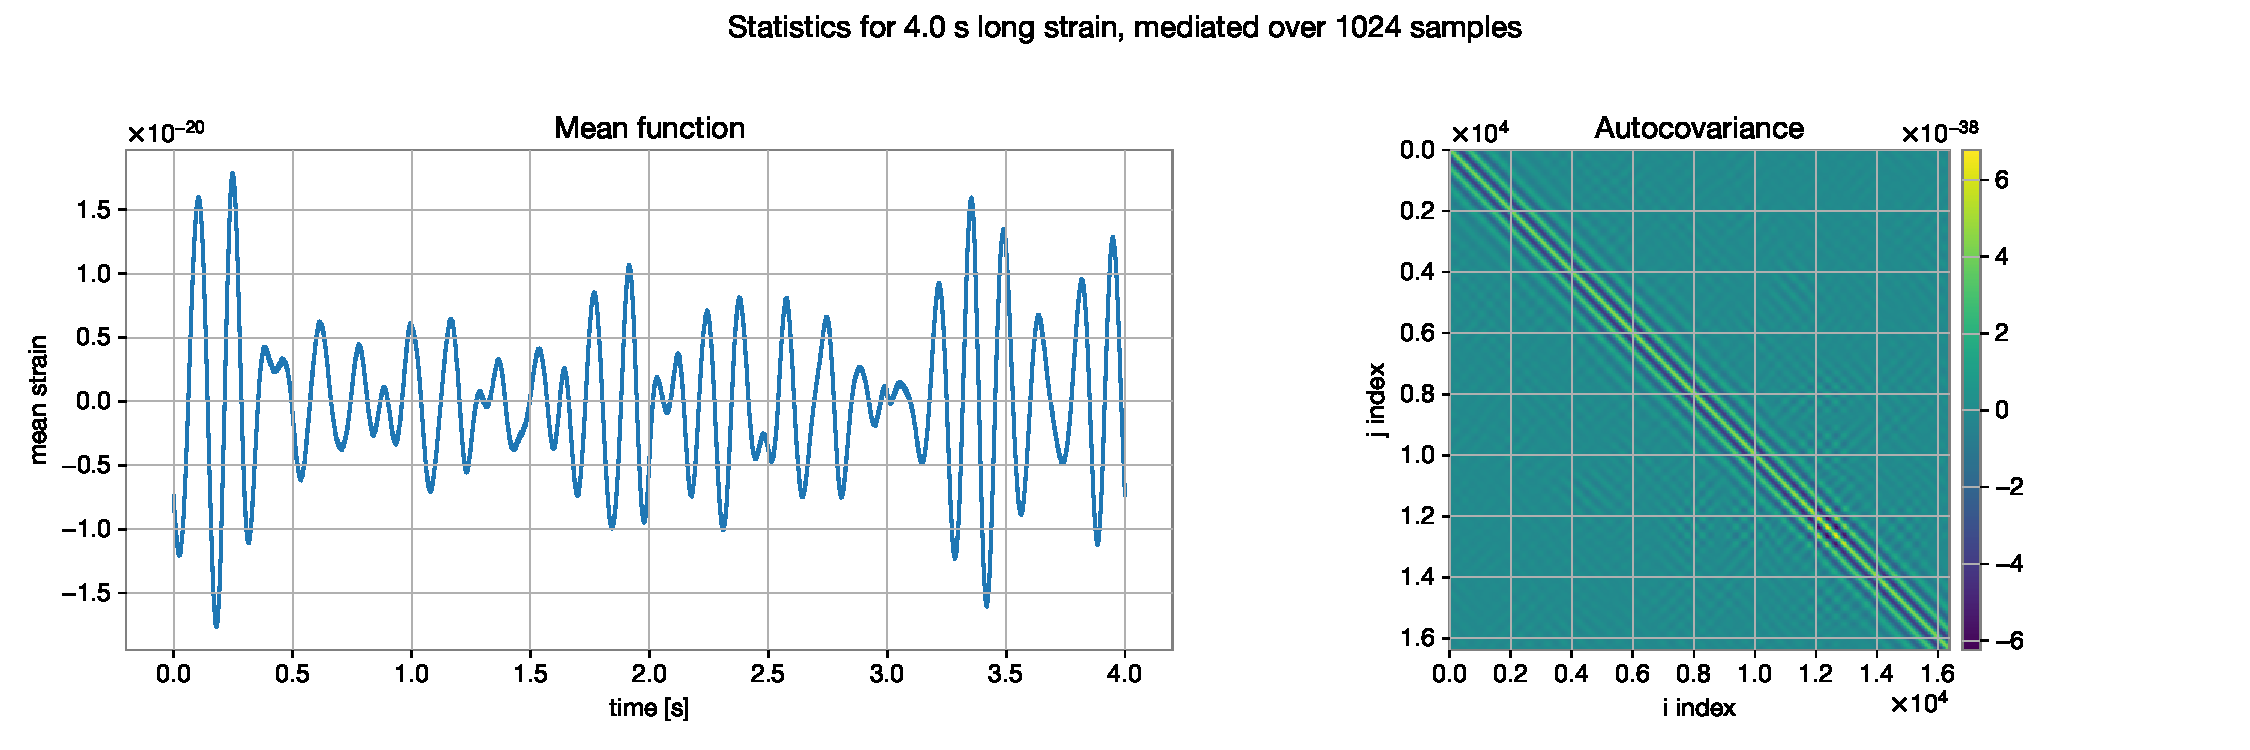
\includegraphics[width=\linewidth]{stat4.0_s.pdf}
    \end{figure}
    The mean is not stationary, but it is two order of magnitude less than the original data $\mathcal{O}(10^{-18})$
\end{frame}

\subsection{Stationarity}
\begin{frame}{Stionarity definition}
\begin{block}{Strongly Stationary Process}
    A process is called strongly stationary iff the statistical properties of every element $t_i$ are the same of a shifted element $t_i+\tau$ $\forall\tau\in\mathbb{N}$.
\end{block}
Roughly speaking, the probability distribution does not change with time, so in particular m(t)=const. and $C(t_i,t_j)=\delta_{ij}\sigma^2$.
\begin{block}{Wide sense stationarity (WSS)}
    A stochastic process is said to be wide sense stationary (WSS) if:
    \begin{itemize}
\item  m(t) is constant

\item  C($t_i,t_j$)=C($| t_i - t_j |$,0) $\forall t_i , t_j \in \mathbb{Z}$
\end{itemize}
\end{block}
    Id est, in a correlation matrix of a WSS process:
    \begin{itemize}
        \item the elements along the diagonal i are the same as the ones in the diagonal -i
        \item all the elements in the same diagonal are equal
    \end{itemize}
\end{frame}

\begin{frame}{Checking for WS stationarity}
In order to check for WSS I define two numbers to be approximatly equal if they are the same up the 5th significant digit.\\
For N=1024 and $\tau=4$ s, our process is not WSS (probably due to the presence of glitches and other frequency lines), but on the timescale $\mathcal{O}$(10 ms) the definition holds
\begin{figure}
    \centering
    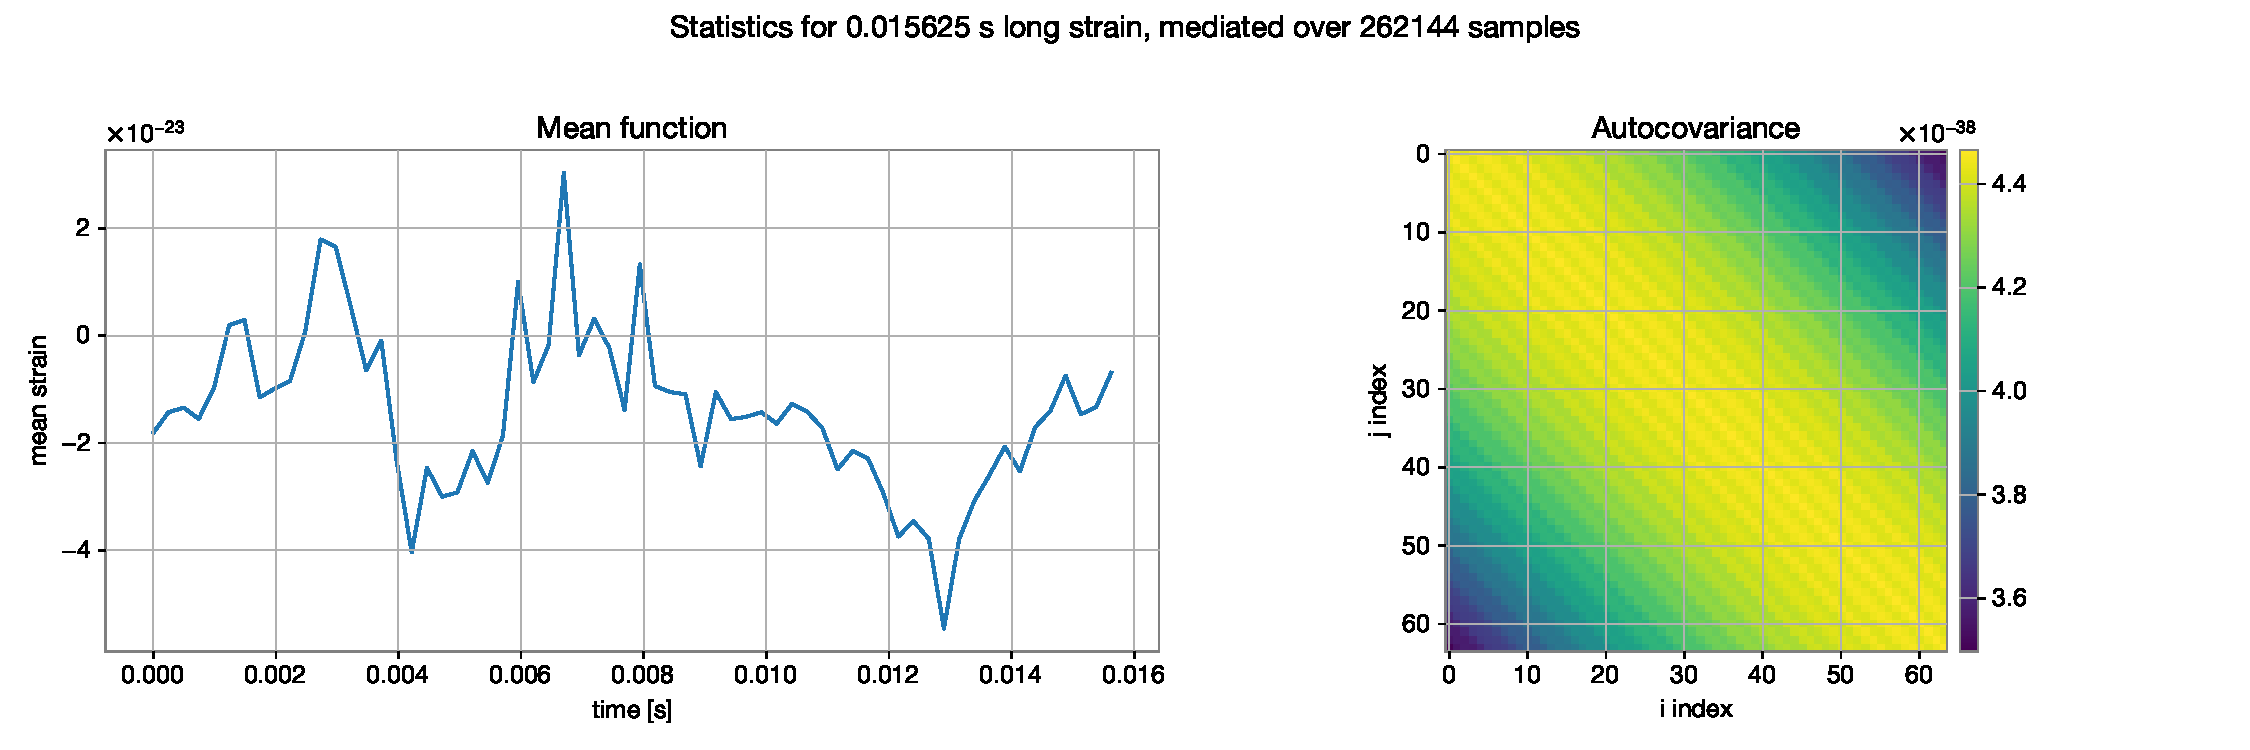
\includegraphics[width=\linewidth]{statWSS.pdf}
\end{figure}
    
\end{frame}
\begin{frame}{ACF}
    Even if not yet demonstrated, we assume WSS for a $\tau = 4 s$ long stochastic process. Under this assumption we can define the (normalized) autocorrelation function as
    \begin{equation}
        C(\tau) = \frac{1}{N \hat{\sigma}^2}\sum_{t=1}^{N-\tau}x_{t+\tau}x_t,
    \end{equation}
    where $N$ is the length of the time series, $\hat{\sigma}^2$ is the estimated variance of the time series and $x_t$ the realization of the time series at time $t$.
    
\end{frame}

\begin{frame}[c]{ACF Plots}
\begin{columns}[onlytextwidth]
	\column{0.48\textwidth}
	\begin{figure}
	    \centering
	    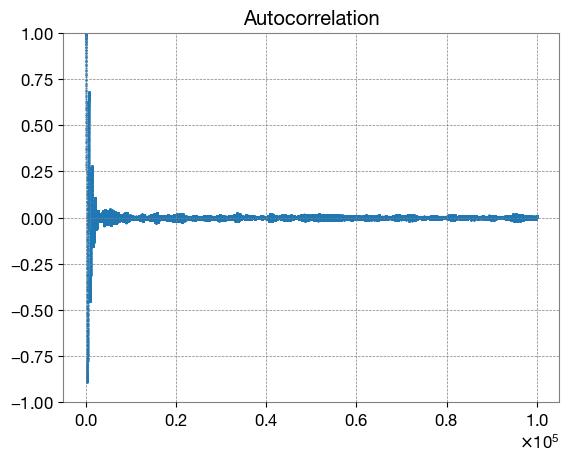
\includegraphics[width=\linewidth]{autocorrelation_whole.png}
	    \caption{First $10^5$ points}
	    \label{fig:whole_acf}
	\end{figure}
	\column{0.48\textwidth}	
	\begin{figure}
	    \centering
	    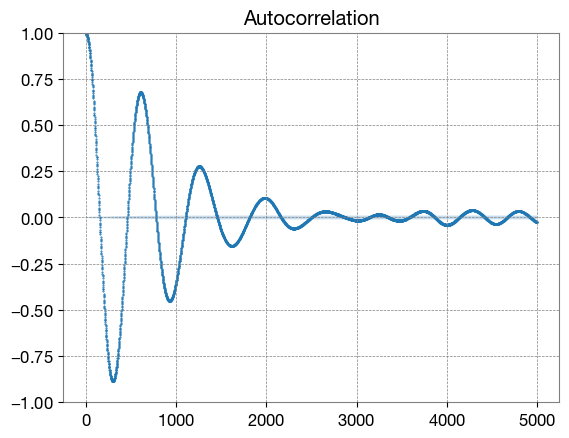
\includegraphics[width=\linewidth]{autocorrelation_5000.png}
	    \caption{First 5000 points}
	    \label{fig:5000_acf}
	\end{figure}
\end{columns}
\begin{center}
The correlations die out before the first second   
\end{center}
\end{frame}

\subsection{Probability distribution}
\begin{frame}{The MaxEnt Principle}
In order to assign a probability distribution we can invoke the Maximum Entropy Principle:
\begin{block}{The MaxEnt Principle}
    The probability distribution which best represents the current state of knowledge about a system is the one with largest entropy, with the entropy being defined as:
    \begin{equation}
        H = -\sum_i p_i \log(p_i)
    \end{equation}
    \end{block}
    \vfill
\begin{columns}
	\column{0.4\textwidth}
The information about our data are:
\begin{itemize}
    \item The process is WSS
    \item \textbf{The mean function} $m(t)=0$
    \item \textbf{The Correlation Matrix} $C_{ij}$
\end{itemize}
\column{0.6\textwidth}
Applying the costrains with the Lagrange Multipliers:
\begin{equation*}
\begin{rcases}
    &\sum_i p_i = 1 \\
    &\sum_i x_i p_i = 0 \\
    &\sum_i x_i x_j p_{ij} = C_{|i-j|}
\end{rcases}\Rightarrow p(\boldsymbol{x}|I) \propto e^{-\frac{1}{2}\boldsymbol{x}^T C^{-1} \boldsymbol{x}}
\end{equation*}
\end{columns}  
\vfill
So the probability distribution is a multivariate gaussian described the autocorrelation matrix
\end{frame}

\begin{frame}{Circulant matrices and their eigenvectors}
Under WSS we can write the autocorrelation matrix as
    \[C=
\begin{bmatrix}
    C(0) & C(\tau) & \dots  & C(N\tau) \\
    C(-\tau) & C(0) & \dots  & C((N-1)\tau)\\
    \vdots & \dots & \ddots & \vdots \\
    C(-L\tau) & & \dots & C(0)
\end{bmatrix}
\]
\begin{itemize}
    \item C is called a Toepliz matrix (i.e. a matrix in which each descending diagonal from left to right is constant)
    \item Toeplix matrices correspond to circulant matrices in the asymptotic limit
    \item And circulant matrices have some nice properties about diagonalization
\end{itemize}
In particular, for a given circulant matrix $C$ it exists a matrix $F$ such that
\[
F^{-1}CF = \text{Diag}\biggl(\sum_{j=0}^{L-1}C_{mj}e^{-2\pi imj/L}\biggr) = \text{Diag}(S_m) = S
\]
\end{frame}
\begin{frame}{PSD and autocorrelation}

$S$ is a diagonal matrix whose elements $S_m$ are the Discrete Fourier Transform (DFT) of the autocorrelation function $C(\tau)$. 
In the continuum, the concept is expressed by 
\begin{block}{The Wiener-Kninchin theorem}
    The autocovariance function C($\tau$) of a stochastically continuous stationary process X(t) may be expressed in term of the power spectral density (PSD) S($\omega$):
    \begin{equation}
        C(\tau) = \int d\omega S(\omega) e^{i\omega t}
    \end{equation}
    
\end{block}
    \begin{block}{PSD (Welch's Method)}
        Distribution of the power (for abstract signals i.e. the square value of the signal) over the frequency domain. It is calculated by splitting the signals into $N_d$ overlapping segments of equal length, then averaging the DFT of the ACF calculated over the segments.
    \end{block}
\end{frame}

\begin{frame}{Simplifying the formula}
In order to simplify the functional form of $p(x|I)$ we can invoke the Wiener-Kninchin theorem and the properties of the circulant matrices:
\[
\boldsymbol{x}^TC^{-1}\boldsymbol{x} = \boldsymbol{x}^T(F^\dag F)C^{-1}(F^\dag F)X = (F\boldsymbol{x})^\dag(FC^{-1}F^\dag)(F\boldsymbol{x}) = \boldsymbol{\tilde{x}}^T S^{-1}\boldsymbol{\tilde{x}}
\]
where $F$ is the Fourier operator, and the $\texttildelow$ denotes a fourier transformed vector.\\
Since $S$ is diagonal, we can finally write the distribution of the noise:
\[
p(\boldsymbol{n}|I) \propto \exp\biggl(-\frac{1}{2}\sum_i \frac{\tilde{n_i}^2}{S_i}\biggr),
\]
i.e. a representation based on independent elements in the frequency domain.
\end{frame}
\begin{frame}{Spectral Leakage and windowing}
    Before taking the DFT, we must account for the possibility of having spectral leakage.
\vfill
    If an analytical signal has no closed form (e.g. it is not periodic over the window) is subject to spectral leakage, i.e. in the frequency domain we find non-analysis frequencies.
    \vfill 
    This can be avoided applying a window, i.e. forcing continuity at the boundaries:
    \begin{columns}
        \column{0.48\textwidth}
        \begin{figure}
            \centering
            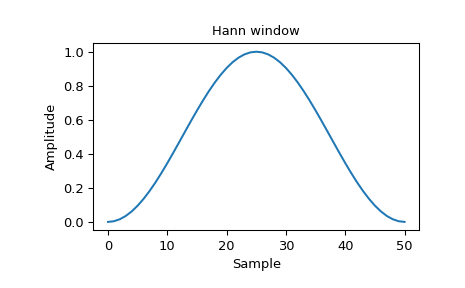
\includegraphics[width=\columnwidth]{hann.png}
            %\caption{Hann Window}
            %\label{fig:enter-label}
        \end{figure}
                \column{0.48\textwidth}
        \begin{figure}
            \centering
            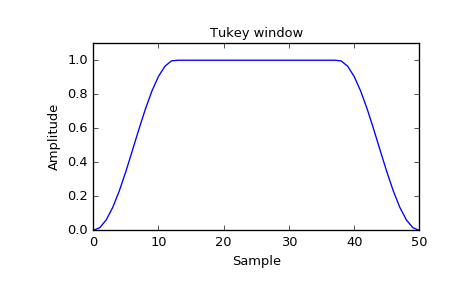
\includegraphics[width=\columnwidth]{scipy-signal-tukey-1_00.png}
            %\caption{Tukey Window}
            %\label{fig:enter-label}
        \end{figure}
    \end{columns}
\end{frame}
\begin{frame}{The Power Spectral Density (PSD) of the noise}

\begin{figure}
    \centering
    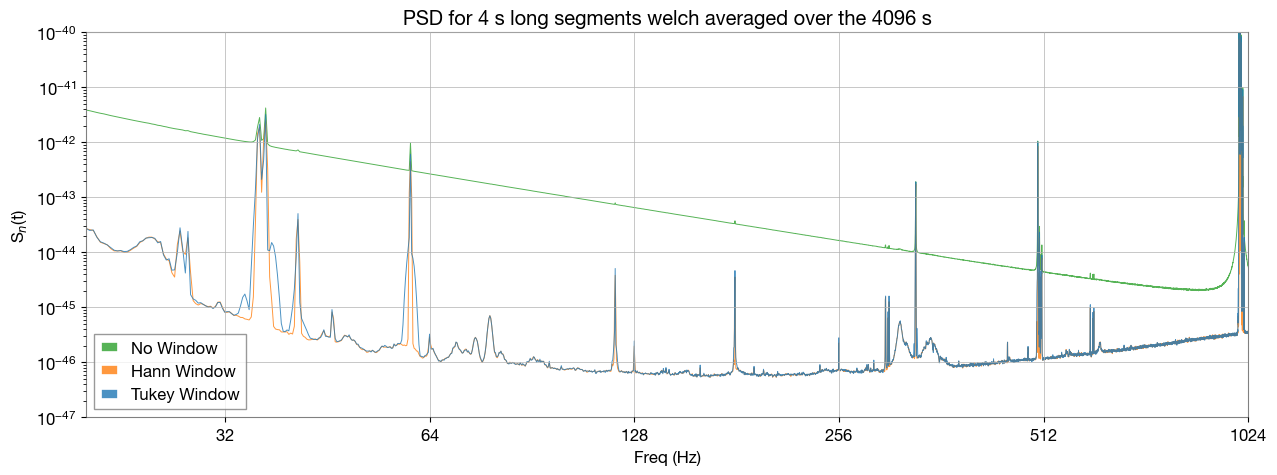
\includegraphics[width=\textwidth]{psd_def.png}
\end{figure}
 \begin{itemize}
     \item Visible trend due to spectral leakage $\Rightarrow$ Window is necessary
     \item Instrumental lines visible
     \item Apart from the spikes, the spectrum resemble a gaussian coloured noise
 \end{itemize}
\end{frame}
\begin{frame}{A simple test for stationarity}
    PSD offers also a good way to test for stationarity:
    \begin{figure}
        \centering
        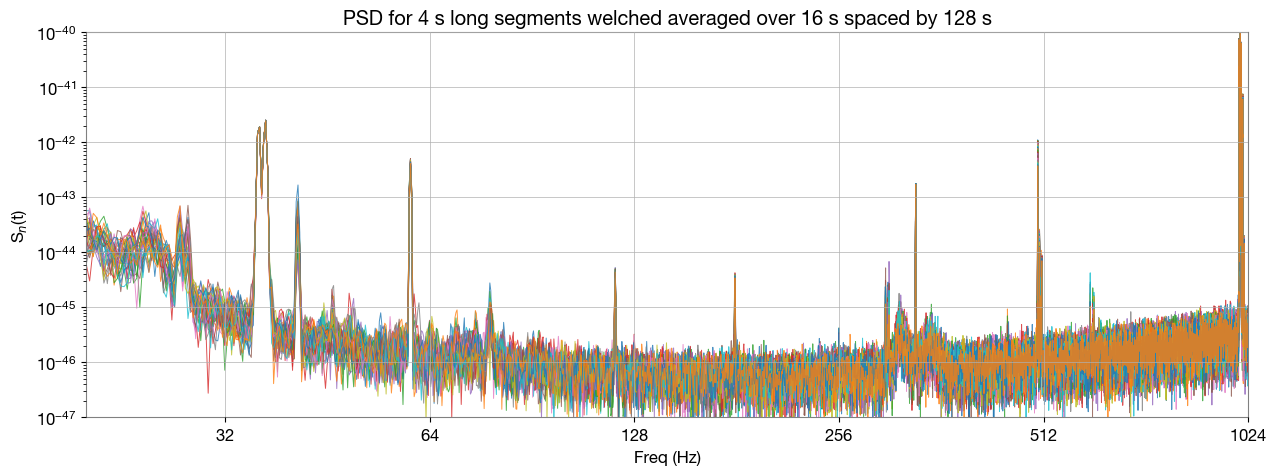
\includegraphics[width=\textwidth]{stationarity_test.png}
        %\caption{Caption}
        %\label{fig:enter-label}
    \end{figure}
    Since the PSD has the same shape for every segment, WSS is a good approximation
\end{frame}

\section{Testing the hypothesis for signal presence}
\subsection{The likelihood}
\begin{frame}{A model for the signal: Taylor F2}
The Taylor F2 model is defined in \textit{Comparison of post-Newtonian templates for compact binary inspiral signals in
gravitational-wave detectors} as 
\begin{equation}
   \tilde{h}(f) = \mathcal{A}f^{-7/6}e^{i\psi(f)}, \quad\text{ with } \mathcal{A}\propto \mathcal{M}^{5/6}/D,
\end{equation}
having called $\mathcal{M}=\frac{(m_1 m_2)^{3/5}}{(m_1 + m_2)^{1/5}}$ the chirp mass and $D$ the luminosity distance. \\

\vfill
Calling $q=m_2/m_1$ the mass ratio, the phase $\psi$ can be expressed in the 2PN approximation as
\begin{align*}
\psi_{2}(f) = &2\pi f t_c - \phi_c - \frac{\pi}{4} + \frac{3}{128q v^5}  \\
&\left[1 + \frac{20}{9} \left(\frac{743}{336} + \frac{11}{4} q\right) v^2 - 16\pi v^3+ 10 \left( \frac{3058673}{1016064} + \frac{5429}{1008} q + \frac{617}{144} q^2 \right) v^4\right]
\end{align*}
in which $v=[\pi (m_1+m_2) f]^{1/3}$ and $t_c, \phi_c$ reference time and phase.
\end{frame}
\begin{frame}{Likelihood}
Defining:
\begin{itemize}
    \item $\boldsymbol{d}$ the full data time series collected by the interferometer;
    \item $\boldsymbol{n}$ the noise in the detector
    \item $\mathfrak{h}$ the gravitational wave signal in the detector (unknown), model by the Taylor F2 model $\boldsymbol{h}$
\end{itemize}
Thus:
\[ \boldsymbol{d} = \boldsymbol{n} + \boldsymbol{h} \Longrightarrow \boldsymbol{n} = \boldsymbol{d}-\boldsymbol{h}\]
And we can write finally our likelihood:
\begin{equation}
    p(\boldsymbol{d}|\boldsymbol{h}, I) = \exp\left(-\frac{1}{2} \left[ \langle \boldsymbol{d} - \boldsymbol{h}, \boldsymbol{d} -\boldsymbol{h} \rangle + \int\ln(S_n(f)) \, df \right] \right),
\end{equation}
where we defined the \textit{noise-weighted inner product} in order to pass to the continuum:
\[\langle a,b\rangle = 2\int_0^{\infty}\frac{\tilde{a}(f)\tilde{b}^*(f)+\tilde{a}^*(f)\tilde{b}(f)}{S_n(f)}df\]
\end{frame}
\subsection{The Matched Filter}

\begin{frame}{The probability of the signal}
Let's define two hypothesis:
\begin{itemize}
    \item $\mathcal{H}_0$: absence of signal (null hypothesis);
    \item $\mathcal{H}_1$: presence of $\boldsymbol{h}$ modeled signal.
\end{itemize}

According to Bayes Theorem:
    \begin{equation}
        p(\mathcal{H}_1|\boldsymbol{d}) = \frac{p(\mathcal{H}_1)p(\boldsymbol{d}|\mathcal{H}_1)}{p(\mathcal{H}_1)p(\boldsymbol{d}|\mathcal{H}_1) + p(\mathcal{H}_0)p(\boldsymbol{d}|\mathcal{H}_0)}=\frac{\mathcal{L}\mathcal{R}}{\mathcal{L}\mathcal{R}+ \frac{p(\mathcal{H}_0)}{p(\mathcal{H}_1)}},
    \end{equation}
    where \[\mathcal{L}\mathcal{R} = \frac{p(\boldsymbol{d}|\mathcal{H}_1)}{p(\boldsymbol{d}|\mathcal{H}_0)}\]
    is the likelihood ratio.
    \begin{exampleblock}{The posterior is monotonic increasing in $\mathcal{L}\mathcal{R}$}
    Being the ratio between the priors $p(\mathcal{H}_i)$ positive, the posterior is monotonic increasing with the likelihood ratio $\mathcal{L}\mathcal{R}$
    \end{exampleblock}
\end{frame}

\begin{frame}{The Matched Filter is the test statistic}
We can analytically write the likelihood ratio:
\[\mathcal{L}\mathcal{R} = \frac{p(d|H_1)}{p(d|H_0)} = \frac{\exp\left(-\langle d - h, d - h \rangle/2\right)}{\exp\left(-\langle d, d \rangle/2\right)},\]
or even better:
\[
\log(\mathcal{L}\mathcal{R}) = \langle d, h \rangle - \frac{\langle h, h \rangle}{2}
\]
 Only the first term of this expression involves the data.  The posterior is monotonic in $\mathcal{L}\mathcal{R}$, and the $\mathcal{L}\mathcal{R}$ is monotonic in  $\langle d, h \rangle$. Thus, $\langle d, h \rangle$ is an optimal test statistic, called \textit{matched filter}.
 
 For the sake of simplicity, let's give it a name:
 \[
\text{SNR} = \rho^2 = \langle d, h \rangle
\]
   
\end{frame}

\subsection{Template Bank}
\begin{frame}{Wavelet generation}
A 4 s long signal wavelet is generated for every configuration of the parameter according to the TaylorF2 model. Then is shifted by a factor $\Delta t = 1/4096 $ s through the whole time series space.
\begin{columns}
    \column{0.48\textwidth}
    \begin{figure}
        \centering
        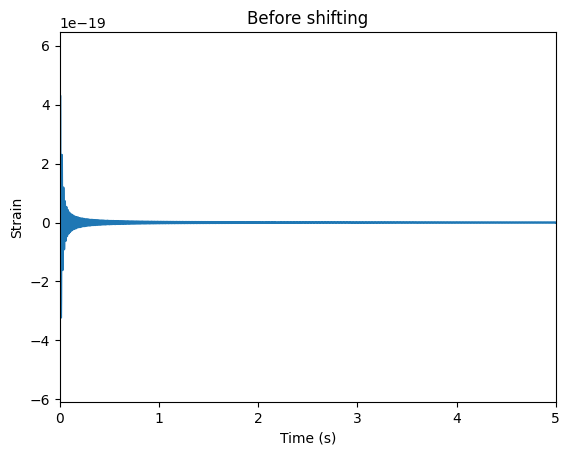
\includegraphics[width=\columnwidth]{before_F2.png}
        %\caption{Caption}
        %\label{fig:enter-label}
    \end{figure}
    \column{0.48\textwidth}
        \begin{figure}
        \centering
        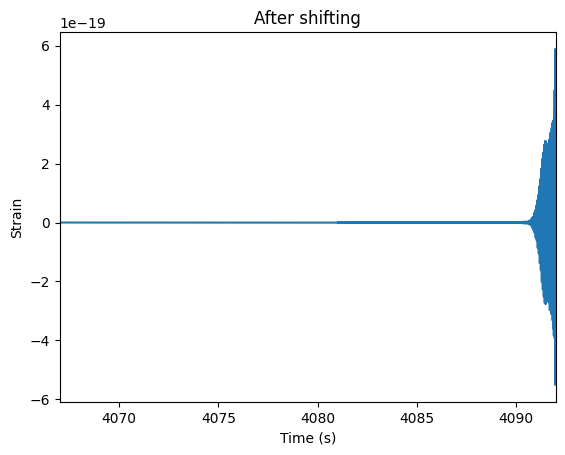
\includegraphics[width=\columnwidth]{after_F2.png}
        %\caption{Caption}
        %\label{fig:enter-label}
    \end{figure}
\end{columns}

\end{frame}

\begin{frame}{Signal to noise ratio}
    For every shift the signal-to-noise-ratio (SNR) - aka our test statistic for the presence of a signal - is calculated. A peak is clearly visible around GPS time 1126259462.4 with a SNR = 17.5.
\begin{figure}
    \centering
    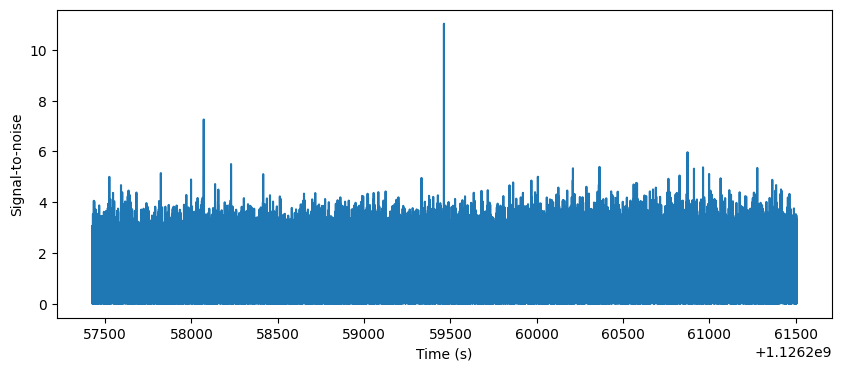
\includegraphics[width=\textwidth]{snr_peak.png}
    %\caption{Caption}
    %\label{fig:enter-label}
\end{figure}
\end{frame}

\begin{frame}{Repetition for every mass candidates}
This process is reapeted for every parameter candidate in range $\mathcal{M} \in [25,35]$ with a $0.1 M_\odot$ step and $q \in [0.5,1]$ with in a $0.01$ step.
\begin{figure}
    \centering
    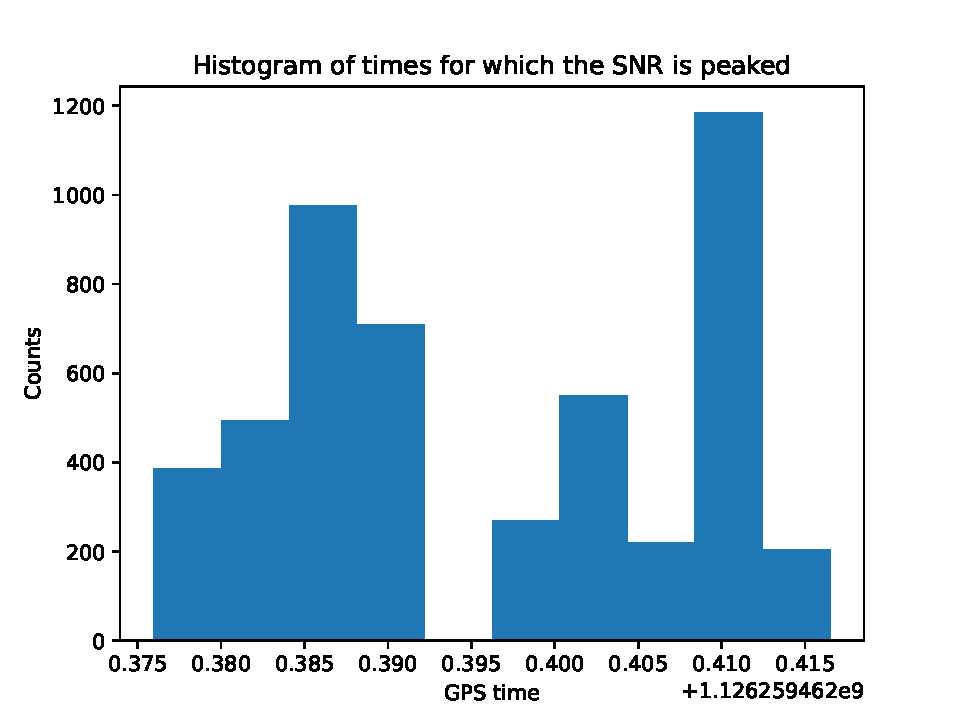
\includegraphics[width=0.8\textheight]{hist_time.pdf}
    %\caption{Caption}
    %\label{fig:enter-label}
\end{figure}
For each of the 5000 samples the time is always consistent with 1126259462.4.
\end{frame}
\section{Parameter Estimation}

\subsection{Prior distributions}
\begin{frame}{Prior of black hole masses}
The model for a Gravitational Wave has potentially 15 parameters (masses, spins, luminosity distance, reference
time and phase, orientation and sky location).
\vfill
For simplicity, we fixed them all and make inference only over the two masses of the binary merger $m_1$ and $m_2$.

We can assume that these are uniformly distributed between 10 and 40 solar masses:
\begin{align}
    p(m_1|I) &\thicksim U(10,40)\\
    p(m_2|I) &\thicksim U(10,40)\\
    \text{with }& m_1 > m_2
\end{align}
It is useful to parametrise the problem in terms of the chirp mass $\mathcal{M}$ and the mass ratio $q$:
\[
    \mathcal{M}=\frac{(m_1 m_2)^{3/5}}{(m_1+m_2)^{1/5}} \qquad
    q=\frac{m_2}{m_1}
\]
where the condition $m_1>m_2$ is shifted to $q<1$.
\end{frame}
\begin{frame}{Prior of chirp mass and mass ratio}
The distribution $p(\mathcal{M},q|I)$ is easily calculated with a change of variables:
\begin{equation}
    p(\mathcal{M},q) = p(m_1(\mathcal{M},q),m_2(\mathcal{M},q))J(\mathcal{M},q),
\end{equation}
 where $J(\mathcal{M},q)$ is the Jacobian of $p$, obtaining:
 \begin{equation}
     p(\mathcal{M},q|I) \propto \mathcal{M}\frac{(q+1)^{2/5}}{q^{6/5}} \quad \text{ with } q<1
 \end{equation}
 Using furthermore the domains of the priors in the $(m_1,m_2)$ space, we get:
 
 \begin{equation}
     p(\mathcal{M},q|I) = \frac{\mathcal{M}}{1079.24}\frac{(q+1)^{2/5}}{q^{6/5}}\mathcal{I}(0.25<q<1)\mathcal{I}(9<\mathcal{M}<35)
 \end{equation}
 
\end{frame}
\begin{frame}{Joint Prior distribution}
\begin{columns}[onlytextwidth]
	\column{0.48\textwidth}
    \begin{figure}
    \centering
    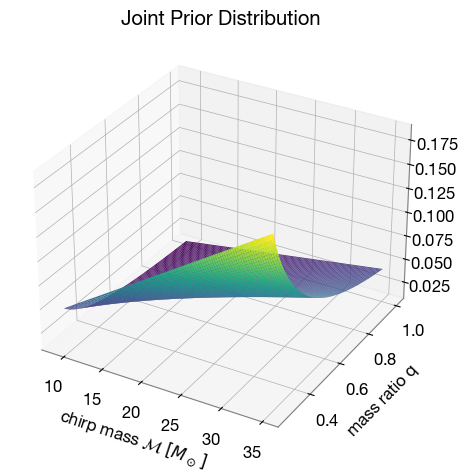
\includegraphics[width=\textwidth]{joint3d.png}
    %\caption{Caption}
    %\label{fig:enter-label}
\end{figure}
\column{0.48\textwidth}
    \begin{figure}
    \centering
    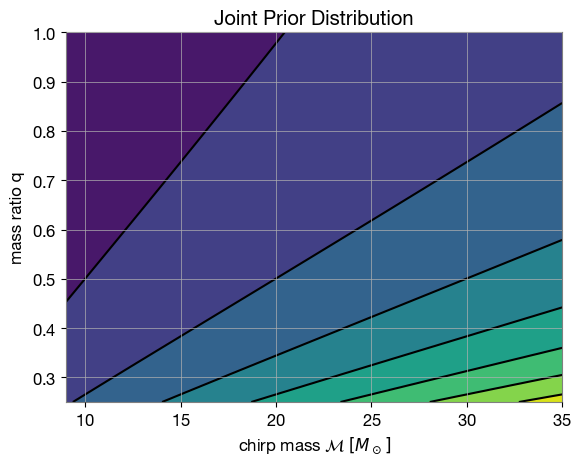
\includegraphics[width=\textwidth]{prior_contour.png}
    %\caption{Caption}
    %\label{fig:enter-label}
\end{figure}
\end{columns}
\end{frame}
\begin{frame}{Marginalized Prior distribution}
We can marginalize over the joint distribution in order to obtain the one dimensional priors
\begin{columns}[onlytextwidth]
	\column{0.48\textwidth}
    \begin{figure}
    \centering
    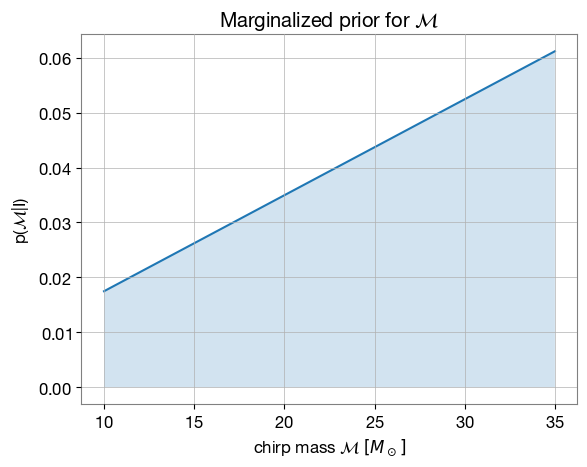
\includegraphics[width=\textwidth]{marginalized_m.png}
    %\caption{Caption}
    %\label{fig:enter-label}
\end{figure}
\column{0.48\textwidth}
    \begin{figure}
    \centering
    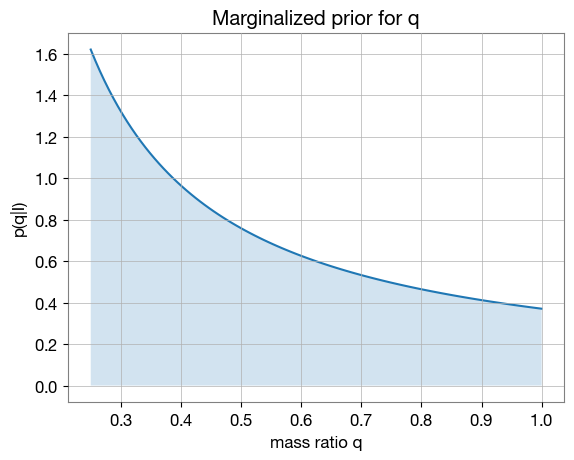
\includegraphics[width=\textwidth]{marginalized_q.png}
    %\caption{Caption}
    %\label{fig:enter-label}
\end{figure}
\end{columns}
\end{frame}
\subsection{Posterior evaluation}
\begin{frame}{The posterior}
    The unknown parameters $\theta=\{\mathcal{M},q\}$ are estimated evaluating the posterior:
\begin{equation}
    p(\theta|d, \mathcal{H}, I) = \frac{p(\theta|\mathcal{H}, I)p(d|\theta, \mathcal{H}, I)}{p(d|\mathcal{H}, I)}
\end{equation}
The prior is defined as
\begin{equation}
     p(\theta|I) = \frac{\mathcal{M}}{1079.24}\frac{(q+1)^{2/5}}{q^{6/5}}\mathcal{I}(0.25<q<1)\mathcal{I}(9<\mathcal{M}<35)
 \end{equation}
The likelihood for the signal hypothesis has already been calculated:
\begin{equation}
    p(\boldsymbol{d}|\theta, \mathcal{H}, I) = \exp\left(-\frac{1}{2} \left[ \langle \boldsymbol{d} - \boldsymbol{h}, \boldsymbol{d} -\boldsymbol{h} \rangle + \int\ln(S_n(f)) \, df \right] \right)
\end{equation}

The evidence $\mathcal{Z}=p(d|\mathcal{H}, I)$ is the real hard value to compute!
\end{frame}
\begin{frame}{Nested Sampling}
    The whole posterior could be approximated with a Markov Chain Monte Carlo, but since the problematic term is the evidence $\mathcal{Z}$ we can turn our attention to the Nested Sampling (NS) algorithm. 
\vfill
In our case we have only two paramaters (we are setting the prior for the other ones to delta functions) but this problem has potentially D=15.
    \vfill
    The great advantage of this method is the fact that we turn a multidimensional problem into a 1-D integral.
        \begin{equation}
        \mathcal{Z}=\int_\Theta d\theta Pr(\theta) \mathcal{L}(\theta) = \int_0^1d\xi\mathcal{L}(\xi)\simeq \sum_i \mathcal{L}(\xi_i)\Delta \xi_i = \sum_i w_i
    \end{equation}
    where $\xi$ is the cumulative prior associated to a contour of $\mathcal{L}$. 

    In this way we also have a "free" way to estimate the posterior as:
    \begin{equation}
        P(\Theta_i) = P(\xi) = \frac{w_i}{\mathcal{Z}}
    \end{equation}
\end{frame}

\begin{frame}{How does NS work? 1/2}
Let's sample $N$ points $x_i$ from the prior, with the constraint $\mathcal{L}>\mathcal{L}_{min}$. We can evaluate the likelihood for each one of these points and order them.

\vfill

The likelihood is inversely related to the prior mass. In fact, the absolute maximum $\mathcal{L}_{MAX}$ correspond to a prior volume equal to zero $\xi_0 = 0$. Following these reasoning, as the likelihood decreases, we could associate an increasingly larger prior mass value, as a smaller likelihood would require broader support.
    \begin{alignat*}{4}
        \mathcal{L}_{MAX} & > \mathcal{L}_N& > &\dots &> \mathcal{L}_0 &> \mathcal{L}_{MIN} \\
0 & < \xi_0 &< &\dots &< \xi_{N} &< 1
    \end{alignat*}
    But  $\xi_i$ are the order statistics of $U(0,1)$, which have known pdf. In particular, 
\begin{equation*}
    f(\xi_{max}) = N\xi_{max}^{N-1} 
\end{equation*}
meaning we can calculate an expected value or even sample from this pdf
\end{frame}
\begin{frame}{How does NS work? 2/2}
\begin{columns}
    \column{0.48\textwidth}
        For calculating the first term in our Riemann sum, we
        \begin{itemize}
        \item take the smallest evaluated likelihood $\mathcal{L}_{0}$ 
        \item Calculate $\xi$, by extracting from $f(\xi_{max})$
        \item Calculate $\Delta \xi = \xi_{N+1} - \xi_N $, where $\xi_{N+1}=\xi_{max}=1$.\\
        \end{itemize}
        \vspace{0.5cm}
        Then, $L_0$ is discarded and a new sample is generated from the prior with the condition $\mathcal{L}>\mathcal{L}_{0}$. \\We repeat the procedure in the previous slide, but now having $\xi_{max} \sim U(0,\xi_{N}<1)$.     \\
        
\vspace{0.5cm}

        We repeated the procedure until a fixed precision is reached.
        
    \column{0.48\textwidth}
    \begin{figure}
        \centering
        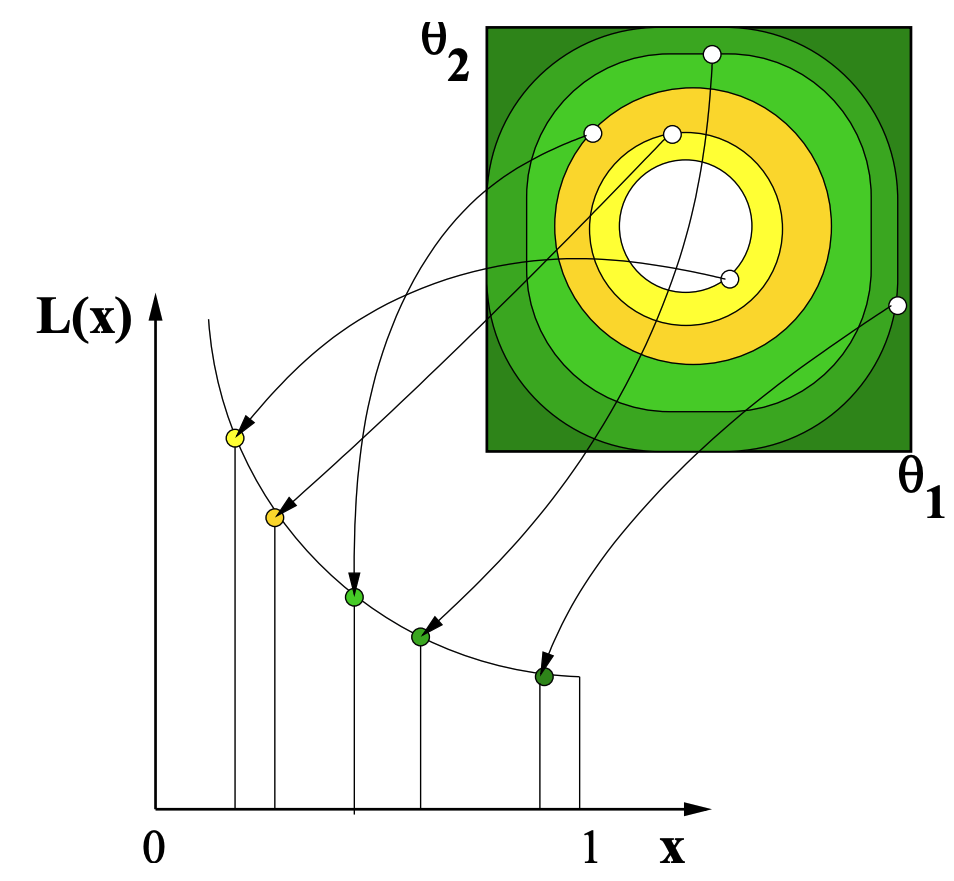
\includegraphics[width=\columnwidth]{NS_scheme.png}
        %\caption{Caption}
        %\label{fig:enter-label}
    \end{figure}
\end{columns}

\end{frame}

\begin{frame}{Model and Hyper Parameters for the Nested Sampling}
\begin{columns}[T]
    \column{0.48\textwidth}
Source Parameters of the Simulated GW150914-like Gravitational Wave Event
    \begin{itemize}
        \item $\mathcal{M} \sim p(\mathcal{M}|I)$ 
        \item $q \sim p(q|I)$ 
        \item $a_1$ = $0.0$ 
        \item  $a_2$ = $0.0$ 
        \item  $d_L$ = $410$ Mpc 
        \item $\phi_c$ = $1.3$ rad 
        \item $t_c$ = $1126259642.413$ GPS seconds 
    \end{itemize}
    \column{.01\textwidth}
    \rule{.01mm}{.7\textheight}
        \column{0.48\textwidth}
Hyper parameters for the nested sampling:\\

\begin{itemize}
    \item sampler: \texttt{dynesty}
    \item $N_{live}=10000$ 
    \item stopping condition: $dlogZ<0.1$
    %\item $N_{step}=100$ minimum number of steps before proposing a new live point 
\end{itemize}
\end{columns}
\end{frame}

\begin{frame}{Estimated Parameter}
Posterior sampled from 29874 samples, with a $\log\mathcal{B}=90.168$.
    \begin{columns}
        \column{0.48\textwidth}
        \begin{figure}
            \centering
            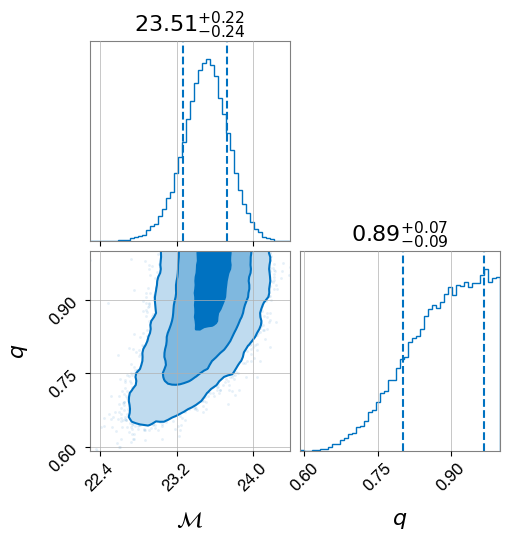
\includegraphics[width=0.8\columnwidth]{param_final.png}
            \caption{Joint and marginal posterior of $\mathcal{M},q$}
            %\label{fig:enter-label}
        \end{figure}
                \column{0.48\textwidth}
        \begin{figure}
            \centering
            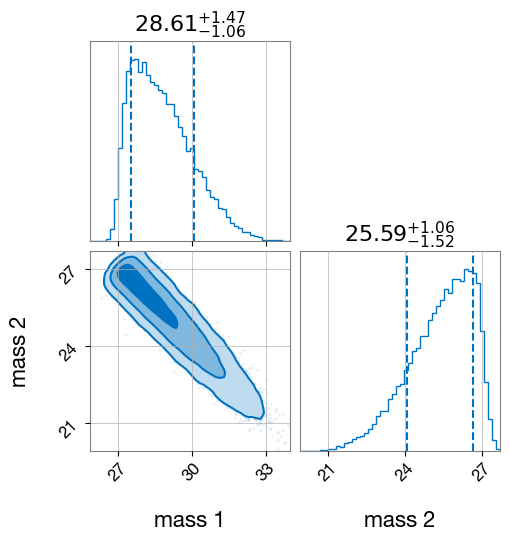
\includegraphics[width=0.8\columnwidth]{param_mass_final.png}
            \caption{Joint and marginal posterior of $m_1,m_2$}
            %\label{fig:enter-label}
        \end{figure}
    \end{columns}
\end{frame}
\begin{frame}{Nested Sampling diagnostics}
    \begin{figure}
        \centering
        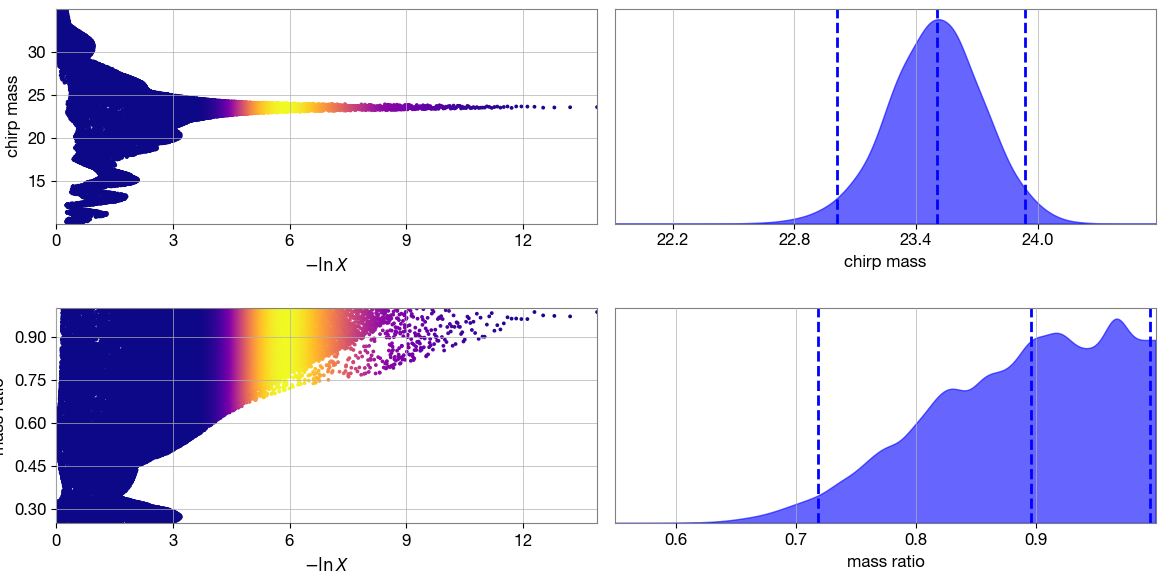
\includegraphics[width=\textwidth]{GW150914_trace_def.png}
        %\caption{Caption}
        %\label{fig:enter-label}
    \end{figure}
\end{frame}
\subsection{Discussion}
\begin{frame}{A test for Nested Sampling}
Toy with generated noise and the same signal as before. In orange values from LIGO and VIRGO.
    \begin{columns}
        \column{0.48\textwidth}
        \begin{figure}
            \centering
            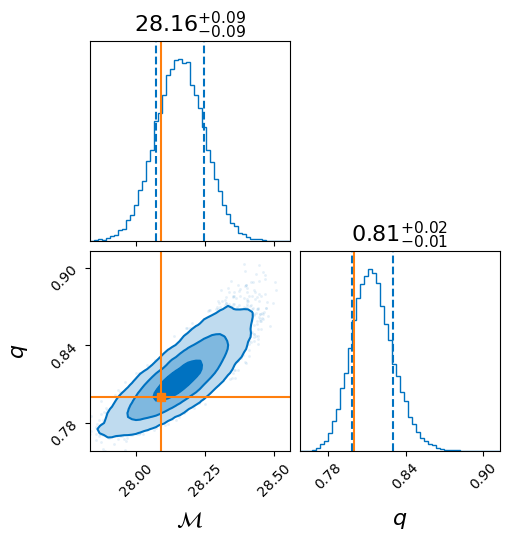
\includegraphics[width=0.8\columnwidth]{def_par.png}
            \caption{Joint posterior of $\mathcal{M},q$}
            %\label{fig:enter-label}
        \end{figure}
                \column{0.48\textwidth}
        \begin{figure}
            \centering
            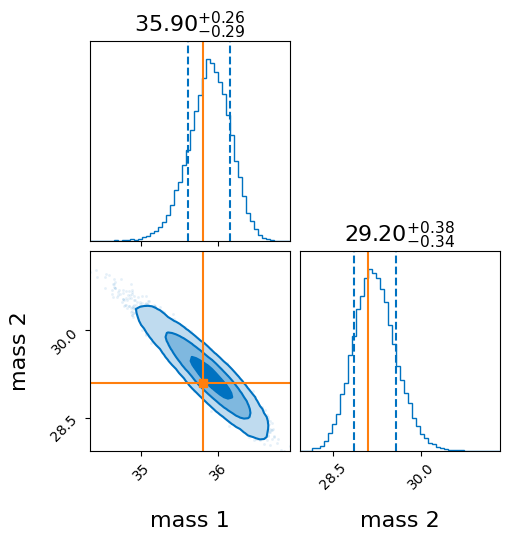
\includegraphics[width=0.8\columnwidth]{mass_par_corr.png}
            \caption{Joint posterior of $m_1,m_2$}
            %\label{fig:enter-label}
        \end{figure}
    \end{columns}
\end{frame}
\begin{frame}{Nested Sampling diagnostics for test}
    \begin{figure}
        \centering
        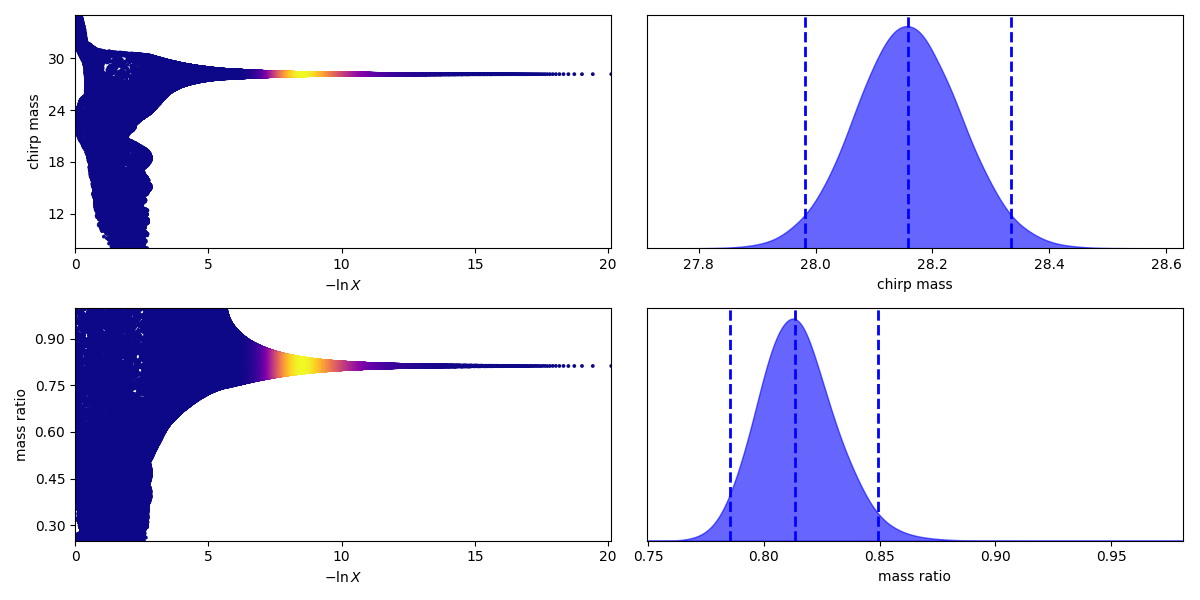
\includegraphics[width=\textwidth]{example_checkpoint_trace.png}
        %\caption{Caption}
        %\label{fig:enter-label}
    \end{figure}
\end{frame}
\begin{frame}{Possible explanation}
\textit{There are in addition a variety of instrumental spectral lines in the data. These include harmonics of the mirror suspension resonances at ~500 Hz; electrical power lines at 60 Hz and harmonics; and calibration lines throughout the spectrum. Such lines are not relevant to the detection or analysis of this event.}
\begin{figure}
    \centering
    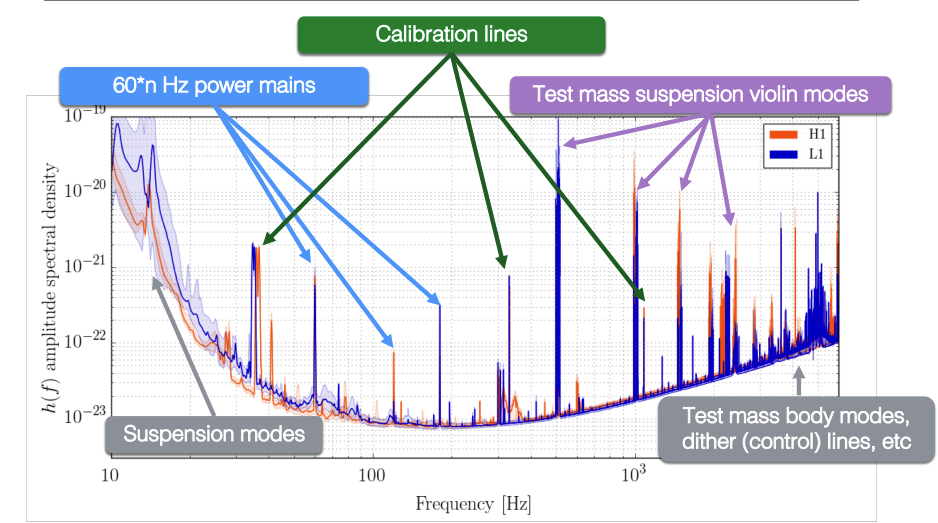
\includegraphics[width=0.6\textwidth]{spectrum_lines.png}
    \caption{Source: \url{https://gwosc.org/techdetails/}}
    %\label{fig:enter-label}
\end{figure}

\end{frame}


\begin{frame}{Final Wave reconstruction}
The signal models are evaluated in our central values for $\mathcal{M}$ and $q$. 
\vfill
    \begin{figure}
        \centering
        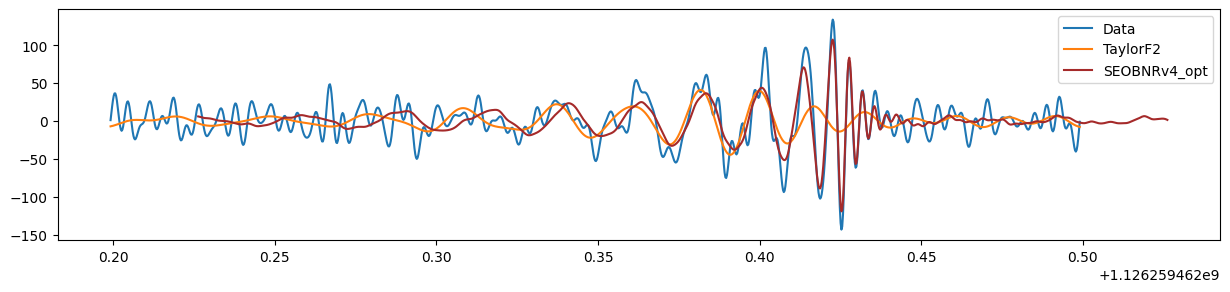
\includegraphics[width=\textwidth]{def_def_gw.png}
        %\caption{Caption}
        %\label{fig:enter-label}
    \end{figure}
    \vfill
    The TaylorF2 is compared to a more complex wave parametrization, yielding a better overlap with the data.
\end{frame}
\begin{frame}{Sum-up}
 In this project I detected a gravitational wave signal (GW150914) in the noisy data stream of the detector. In particular,
\begin{enumerate}
    \item I modelled the noise a WSS stochastic process
    \item I calculated the probability distribution of the stochastic process (a.k.a. our likelihood) using the MaxEnt Principle
    \item I used the Wiener-Kninchin Theorem to simplify the calculation of the likelihood
    \item I derived the test statistic for the detection of the GW, which was the Matched Filter
    \item I generated a Template Bank for different mass candidates evaluating the time for which the signal-to-noise ratio was highest
    \item I performed a nested sampling in order to evaluate the posterior of the parameters and make an inference about their values
    \item I tried to provide an explanation for the discrepancies of the values with the literature
\end{enumerate}
    Although the estimated mass values are not comparable with the ones in literature, they are the same order of magnitude
\end{frame}
% Thank you page
\beamertemplateshadingbackground{structure.fg!90}{structure.fg}
\begin{frame}[plain]
	\vfill
	\centering
	{
		\centering \Huge \color{white} Thank you for your attention%\\[10pt]Questions?
	}
	\vfill
\end{frame}

\end{document}



